\begin{figure}[h!]
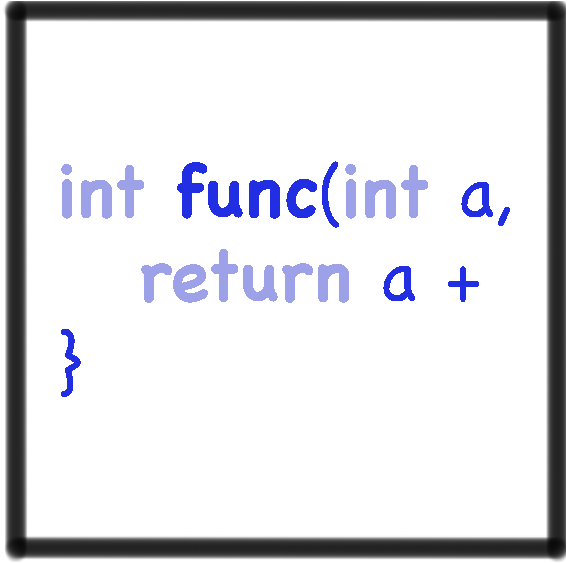
\includegraphics[width=0.2\textwidth]{img/assnType_4}
\end{figure}

The use of neural networks to learn a joint embedding space is useful for introductory control flow assignments. However for general programs that students would write in an undergraduate programming course, networks which represent recursive structures (such as programs) are currently not powerful enough to be the basis for understanding the space of student partial solutions.

In this chapter we develop a way to understand partial solutions for general programming assignments. To do so we decompose online homework submissions into a vocabulary of ``code phrases'', and based on this vocabulary, we architect a queryable index that allows for fast searches into the massive dataset of student homework submissions. To demonstrate the utility of our homework search engine we index over a million code submissions from users worldwide in Stanford's Machine Learning MOOC and (a) semi-automatically learn shared structure amongst homework submissions and (b)  generate specific feedback for student mistakes. 


\mypara{Search engines for student submitted content}
\looseness -1 %\Chris{This seems to repeat many thoughts from previou sections: 
%There has never existed as pressing a need to efficiently search student online content before.
%But 
With the amount of collected student content increasing at a growing rate
	and the lines between formal classroom learning and informal online learning quickly blurring, 
		search engines for student submitted content seem inevitable, and potentially enormously valuable. 
		%\Chris{this seems like a good place to define what a search engine over homework means. There is a medium intellectual jump between these two sentences}
		These search engines would allow one to explore a massive number of homework submissions by efficiently retrieving submissions matching specific criteria.
Students would then benefit by being able to look for other students who think alike,
			 to see how students with different viewpoints think,
			to find alternative strategies of approaching a homework problem,
			or simply to browse other work for inspiration.
			%\Chris{What about getting feedback? I know its coming... but its not clear here.}
Instructors, on the other hand, would also benefit %, for while an instructor cannot read through tens of thousands
%of student submissions to a MOOC,  she can 
by being able to query a search engine in order to look for submissions of a particular
			type or even to count the number of students who submitted the same
			or a similar class of solutions.
%In this paper, we present a system capable of searching for programming code among a massive collection of submissions to a MOOC. Even though our focus is on code, we believe that similar ideas can have broad impact on a variety of courses beyond computer science.

\looseness -1 While search engines for code have existed for a number of years (see~\cite{paul94,thummalapenta07,hummel08,kim10}),
the nature of MOOC datasets makes for a setting that is quite distinct from that of typical code search.
%Even though one would still need to comb through massive amounts of code, 
In the MOOC setting there is significantly more structure, since
(1)  submissions often take the form of single unit-testable functions written in a single language, and (2) 
all students submit attempts of the same problem at the same time.   
Due to this similarity between many submissions, 
it is possible to exploit the shared structure of multiple submissions in several ways.
For example, this shared structure allows one to reason about the
semantics of code and the intentions of the programmer.   
%\Jon{[DELETE] And of course while it would be nice
%to understand programmer intent in general code, the problem is more important for students who are potentially
%just beginning to learn to code.}


\looseness -1 The engine that we propose in this chapter is built around a massive index over the existing student code submissions
which can be searched using a variety of queries and supports a number of possible applications such as (but not limited to)
finding alternative implementations, mining common approaches and misconceptions, and providing personalized feedback.
%\Jon{Chris?}
Codewebs is designed to be highly scalable, allowing us to
find and leverage shared structure amongst submitted programs and is able to reason about semantically similar student code.
The main power of our system stems from its ability to tailor the way it deals with code semantics to each homework problem individually.
% deals with code semantics is specifically tailored to each homework problem, but 
Specifically, we
utilize existing data to learn about each homework problem rather than requiring an excessive amount of human effort for each problem.
Finally, the Codewebs system is designed so as to be easily portable to diverse programming assignments
and to different programming languages remaining cognizant to the fact that instructor time is a limited resource.
%Our system is 

\mypara{Delivering scalable human feedback}
Instructor time is also a limiting factor in delivering feedback to students, which is critical for learning.
%Another issue in online education that the Codewebs engine addresses is that of allowing a human to scalably deliver feedback.
With the number of engaged students in a MOOC commonly exceeding ten thousand, many benefits of face-to-face instruction are easily lost.
Even despite the fact that programs can be checked for correctness (i.e., unit-tested) automatically, coding assignments are complex in that they can 
be approached with a multitude of algorithms or strategies and typically require creativity. 
Thus in many coding problems, students can benefit from more feedback than a binary ``correct vs. incorrect''.   
It is difficult, however, to gauge student understanding without being able to personally peruse through  tens of thousands of code submissions.
And it is consequently difficult to grade student work, to provide detailed student feedback, or respond to individual questions. 

\looseness -1 Detailed assignment feedback is in general neither easily automated or even appropriate for typical crowd-sourcing platforms such as Mechanical Turk since graders are required to have a certain level of expertise.  One proposed solution (pursued, for example, by the Coursera platform) has been to use peer grading instead, allowing students to grade each other. While peer grading has shown signs of initial success, it also suffers from a number of limitations including inconsistencies and biases amongst peer graders as well as sometimes an unwillingness or inability to provide high quality and constructive feedback \cite{piech13}.

%\looseness -1 Among the many automated and crowdsourcing approaches now available, 
%we take the view that \emph{human instructors still have a key role to play, even in the global classroom}.
%Seamlessly incorporating human feedback into the loop would be both desirable to instructors and beneficial for students.
Our method for providing scalable human feedback derives from the observation that even though there may be many thousands of unique submissions to an open-ended programming assignment the diversity reflects a much smaller number of compounded student-decision points. By recognizing ``shared parts" of student solutions and decoupling different decisions, instructor feedback can be force multiplied. The idea behind our tool is to have an instructor provide detailed feedback only on a handful of submissions which we can intelligently propagate to new solutions via underlying assignment structure learned using our homework search engine. We aim to create a system where a teacher can provide detailed 
feedback for thousands of students with the same effort that she would spend in an ordinary college course.

The strategy of propagating teacher feedback aligns with our view that \emph{human instructors have a key role to play in the future digital classroom}. Seamlessly incorporating human feedback into the loop bridges the gap between the typical MOOC experience and the small classroom experience.
 Finally, because our system discovers the commonalities amongst student submissions using the corpus of students submissions, adding more student data to our data bank
 will improve our statistical confidence and coverage, 
 allowing us to provide meaningful feedback to more students, detect more classes of conceptual errors, and generally improve the utility of our system.

%And by employing the Codewebs engine as a force multiplier, 
%\Jon{We discuss how the Codewebs  engine can  allow for a teacher to provide detailed 
%feedback for thousands of students but with the same effort that she would spend providing 
%feedback to students in an ordinary college course.  In a nutshell, our method works 
%by allowing an instructor to provide
%detailed feedback only on a handful of submissions (or parts of submissions), which we intelligently  propagate to new submissions
%along the ``shared parts'' that the Codewebs system is good at detecting.
%We believe that our system can thus help as a ``force multiplier'' for human instructors who would like to
% bridge the gap between the typical MOOC experience and the small classroom experience. Finally, continually adding student data to our data bank
% will improve statistical confidence and coverage, 
% allowing us to provide meaningful feedback to more students and detect more classes of conceptual errors, and generally improve the utility of our system.}

\mypara{Overview of main contributions}
To summarize, we propose in this paper a novel system, \emph{Codewebs}, for searching through code
submissions to a programming intensive MOOC as well as a methodology for scalably providing
human level feedback to students in the MOOC.
%Our system is fast, makes few assumptions and requires minimal assistance from human instructors.
%More broadly, we believe that search engines for student content are naturally going to be part of the future of
%online learning at scale--and may even be adapted for other web contexts.
%
%\looseness -1 There are several broad technical issues at the core of our system.  First, how to quantify similarity between source code is a notoriously difficult problem.
%In the educational setting, it is particularly crucial to measure similarity not just in syntax, but in semantics and even intention.
%Second, how to seamlessly incorporate human feedback into the loop is desirable to instructors and beneficial for students.
%The final issue is how to scale to courses with  tens of thousands of submissions per programming problem 
%(including indexing and giving of human feedback, and quantifying similarity) --- a problem which will only become
%more difficult as students continue to take the same courses online and as MOOCs become more popular.
%%In this paper we address all of the above issues, proposing highly scalable algorithms for indexing by subtree, subforest, and context, as well as
%%a method for data-driven discovery of  equivalence classes of subtrees/forests which allow users to search for code by semantic similarity.
%%We show that information from a human instructor can be used to facilitate bug understanding as well as to give feedback.
The main technical innovations that we have developed are as follows.
\begin{itemize}
\item We propose an efficient method for indexing code by ``code phrases'' corresponding to constituent parts
of code submissions to a massive scale programming course.  In particular, we introduce a novel way to query for the surroundings, or \emph{context} of a code phrase, 
which allows us to reason about the behavior of code within its context.
\item We develop a data driven approach for automatically finding semantically equivalent code phrases.
In particular we introduce a notion of \emph{probabilistic semantic equivalence} allowing
us to connect syntax with semantics and to compare code with respect to both.
\item We demonstrate applications of our search index
such as bug finding (without having to execute code) and 
allowing a human instructor to  provide feedback at MOOC scales.
\item We demonstrate the scalability of the Codewebs engine and show results on code submissions to a real MOOC, Stanford's machine learning course,
which  had over 120,000 students enrolled worldwide, who submitted over a million code submissions in total.
We also explore the variability of this dataset, showing in particular that the frequency counts of  
student submitted code phrases for a single programming problem follow a Zipf law distribution despite the
fact that all submissions are implementations of the same function.
\end{itemize}
\begin{table}[t!]
\center
\begin{tabular}{|c|c|}
\hline
   \# submissions in total & 1,008,764 \\
   \# coding problems & 42 \\
    Average \# submissions per problem & 24,018 \\
    Average \# students submitting per problem & 15,782 \\
    Average \# of lines per submission  & 16.44 \\     %(discounting starter code)
    Average \# of nodes per AST & 164 \\
%    Fraction of correct submissions & 1 \\
    \hline
\end{tabular}
\caption{Statistics of the ML class dataset. }
\label{tab:datasetsummary}
\end{table}
\begin{figure*}[t!]
\center
\subfigure[]{
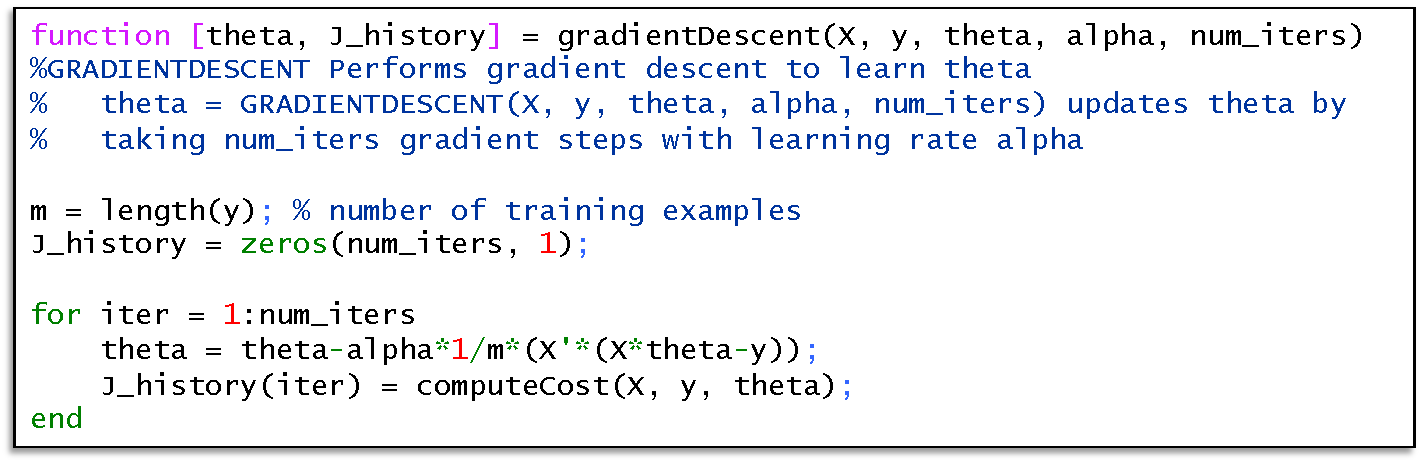
\includegraphics[width=.33\textwidth]{img/goodimplementation.pdf}
\label{fig:codeexample}
}
\subfigure[]{
\raisebox{3mm}{
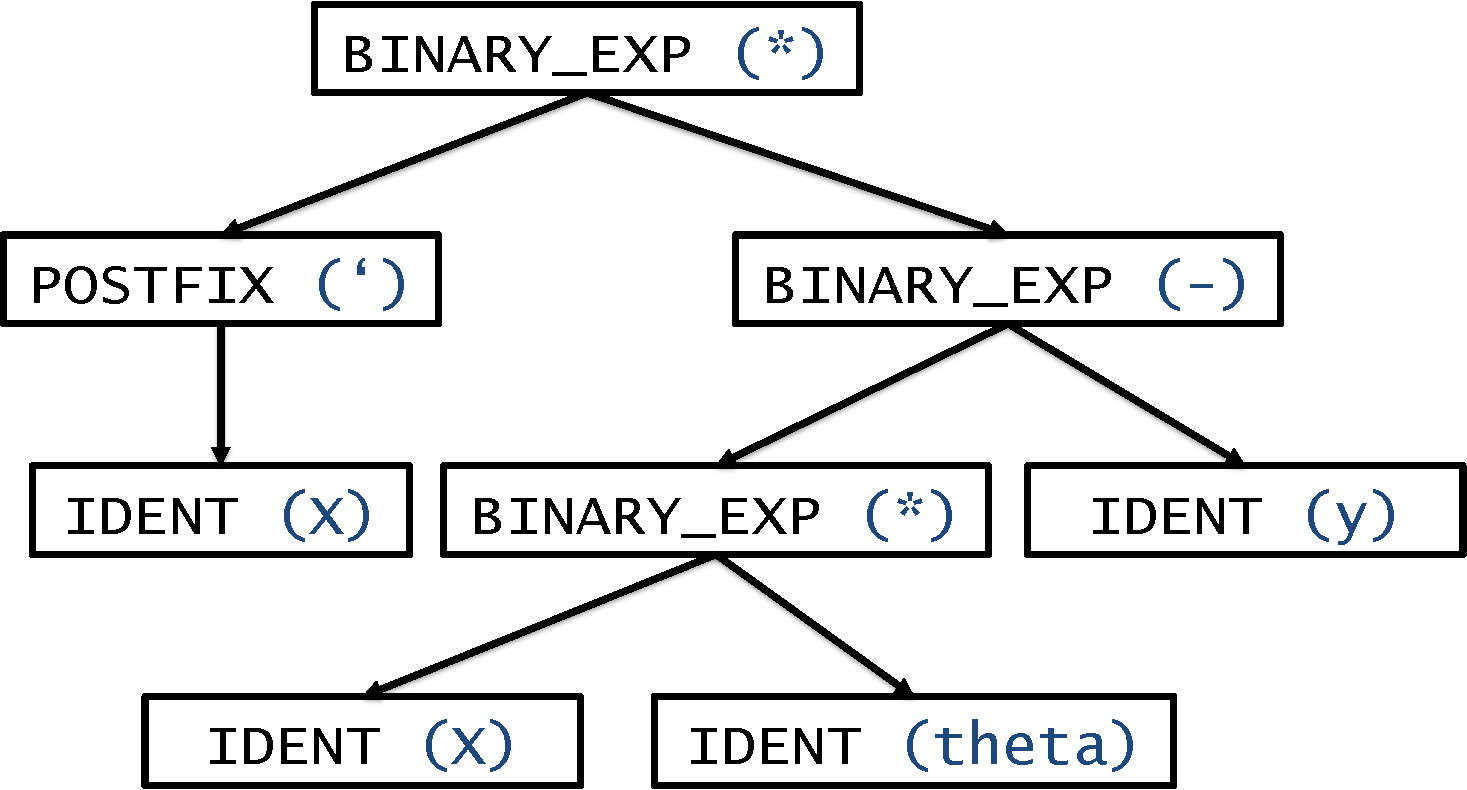
\includegraphics[width=.21\textwidth]{img/astexample2.pdf}
}
\label{fig:astexample2}
}
\subfigure[]{
\raisebox{8mm}{
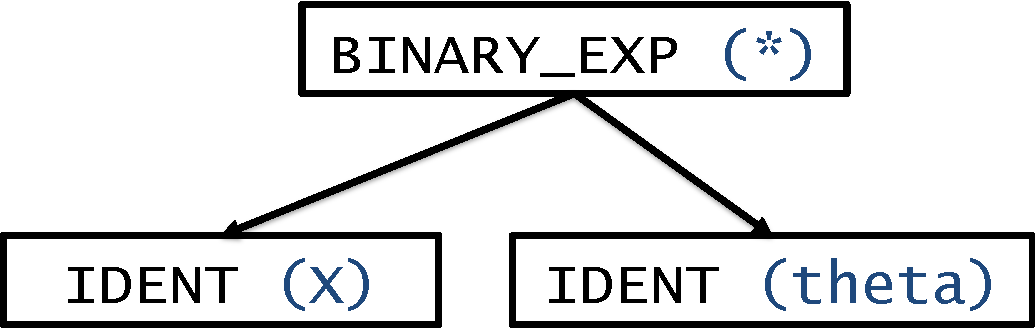
\includegraphics[width=.13\textwidth]{img/subtreeexample.pdf}
}
\label{fig:subtreeexample}
}
\subfigure[]{
\raisebox{3mm}{
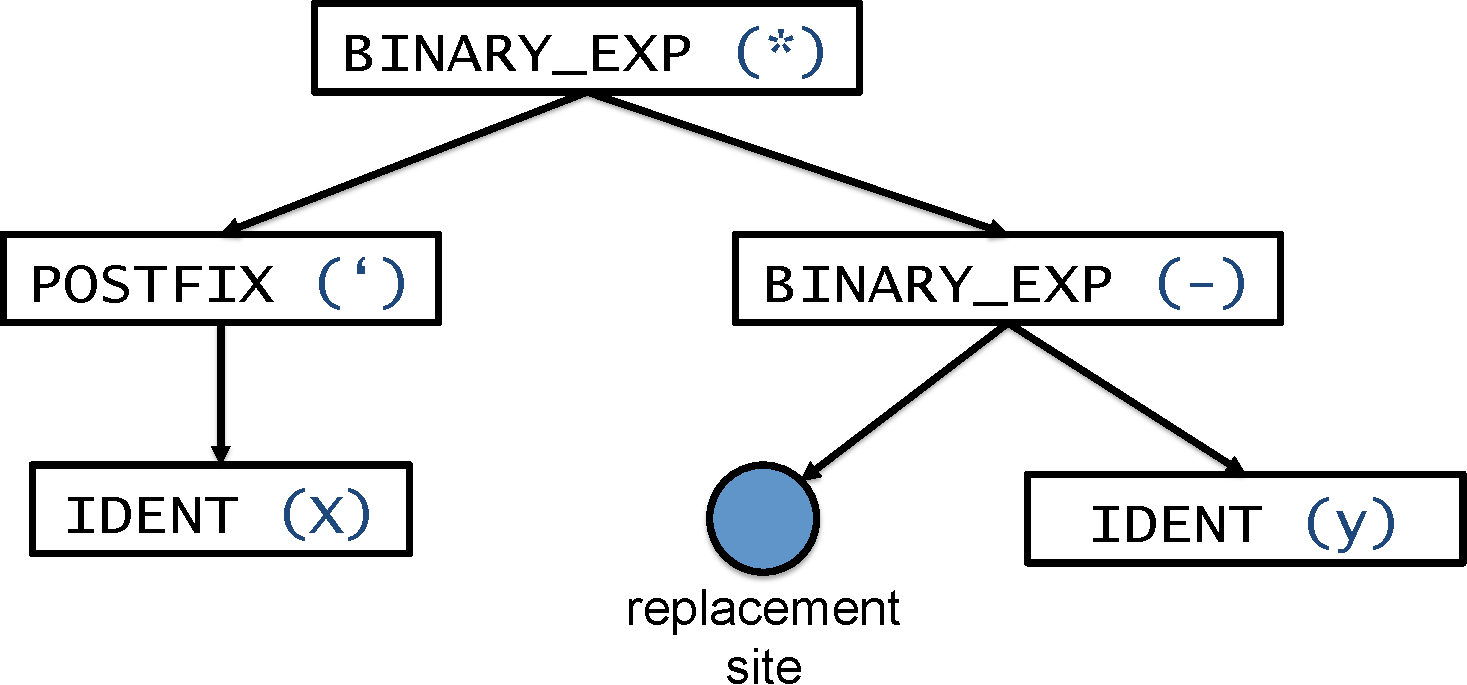
\includegraphics[width=.21\textwidth]{img/contextexample.pdf}
}
\label{fig:contextexample}
}

\caption{
\subref{fig:codeexample} Example code submission to the ``Gradient descent (for linear regression)'' problem;
\subref{fig:astexample2} Example abstract syntax tree for linear regression gradient expression: $X'*(X*\theta - y)$;
\subref{fig:subtreeexample} Example subtree from the AST from Figure~\ref{fig:astexample2}; \subref{fig:contextexample} 
Context of the subtree with respect to the same AST.  Note the additional node denoting the ``replacement site'' of the context.
}
\end{figure*}



\section{Data from a programming intensive MOOC}\label{sec:dataset}
We showcase our Codewebs system using data collected from 
Stanford's online machine learning (ML) Class (taught by Andrew Ng), 
which opened in October 2011 with over 
120,000 students registering. Over the duration of the course,
over 25,000 students submitted at least one assignment, and 
10,405 students submitted solutions to all 8 homework assignments.  Each
assignment had multiple parts (which combined for a total of 42 
coding problems), in which students were asked to implement algorithms covered in lectures such as regression, neural networks and support vector machines.
Code for the ML class was predominantly written in Octave, a high level interpreted language similar to MATLAB,
and the submissions collectively covered nearly all of Octave's basic language features.
Submissions to the course website were assessed via a battery of unit tests where the student
programs were run with standard input and assessed on whether they produced
the correct output. 
We remark that high level languages such as Octave are fairly popular for instruction because they
allow a student to ignore many of the low level frustrations associated with programming and 
concentrate on the more important higher level concepts.
But they are also harder languages to automatically analyze due to their more flexible syntax and dynamic typing.
As we show in this paper, data driven methods give us a way to effectively analyze submissions in such languages.

\looseness -1 Figure~\ref{fig:codeexample} shows a correct attempt at the ``Gradient descent (for linear regression)'' problem
assigned in the first homework.  In this problem, students were asked to find a linear predictor of the output vector $\texttt{y}$
based on the input matrix $\texttt{X}$. Throughout the paper, we will use this linear regression coding problem as a running example.

\looseness -1 The Codewebs engine allows us to efficiently query this massive collection of code 
submissions from Stanford's ML class, all of which attempt to implement the same functionality.  With so many submissions of the same 
programming problem, we are able to obtain a dense sampling of the solution space, in which 
 we observe almost every conceivable way of approaching the problem both correctly and incorrectly.
The dataset is thus perfect for highlighting the advantages of Codewebs which is able to exploit large amounts of data to do things 
that would be much more difficult to accomplish otherwise.
At the same time, a massive course such as ML class can greatly benefit from a detailed student feedback tool, 
making our dataset also ideal for demonstrating the applicability of Codewebs.
More statistics of our dataset are summarized in Table~\ref{tab:datasetsummary}.

	
\mypara{Structured representations of syntax} 
\looseness -1 In addition to a string representation of each student's code submission,
we parse each student submission into an \emph{abstract syntax tree (AST)} representation. 
Each AST (which is equivalent to that created internally by the Octave software~\cite{eaton97}) 
is stored explicitly in our database in JSON format.   An example AST is depicted in Figure~\ref{fig:astexample2}.
Running on the ML class dataset, our parser accepts over 99.5\% of  submitted code, failing in 
a small percentage of cases (often due to submissions in different languages such as Python or MATLAB),
which we discard from the dataset.  
Nodes in our ASTs are specified by a \emph{type} (e.g., $\nodeSTATEMENT$, $\nodeASSIGN$) and an optional \emph{name} (e.g., $\texttt{X}$, $\texttt{theta}$, 
$\texttt{gradient}$). 
Other than the statement and identifier nodes, we do not assume any specific knowledge of the semantic meanings of node types.

\looseness -1 Reasoning with abstract syntax trees instead of the original source code allows the Codewebs system to effectively ignore
cosmetic idiosyncrasies in whitespace, comments, and to some extent, differences in variable 
names.   We find in many cases that multiple submissions that are distinct as code strings can correspond to the same AST.
Thus after parsing, we retain just over half a million distinct ASTs from the original million submissions along with the number
of occurrences of each unique AST.  

\section{Efficient Indexing of code submissions}\label{sec:indexing}
\looseness -1 What basic queries or items should a code search engine index?
If we viewed code simply as a string, it would be reasonable to query by terms, or phrases or regular expressions,
but with the additional tree structure of our ASTs, we can go beyond traditional ``flat'' queries.
The Codewebs engine accepts basic queries in the form of what we call \emph{code phrases}, subgraphs of an AST
which take three forms: subtrees, subforests, and contexts, which we now define.  In the following, consider any AST denoted by $\AST$:

{{\noindent \bf [Subtrees]}} \emph{Subtrees} represent the most basic form of code phrases and 
are specified by a single node $\node$ in AST $\AST$ and contain all descendants of $\node$.
If an AST $\mathcal{B}$ is a subtree of AST $\AST$, we write $\mathcal{B} \leq \AST$.
When referring to a specific subtree rooted at a node $\node$ of an AST, we write $\subtree$.

{{\noindent \bf [Subforests]}} In addition to subtrees, we consider \emph{subforests} which capture everything in a contiguous sequence of statements.
Specifically, we define a subforest to be a consecutive sequence of \emph{statement subtrees} (i.e., 
subtrees rooted at $\nodeSTATEMENT$ nodes).  

{{\noindent \bf [Context]}} Because the function of a code snippet generally depends strongly on the surrounding region of code in which it appears,
we also allow for these surroundings to be directly queried by our engine. 
Formally, we define the \emph{context} of a subtree $\subtree$ within a larger subtree $\subtreeprime$ of the same AST
to be the subgraph of $\subtreeprime$ which does not contain anything in $\subtree$ to which we add an additional leaf attached to the parent of $\node$,
representing the ``replacement site'' where other subtrees could potentially be swapped in.
For example, the context of the body of a for-loop with respect to the subtree rooted at that for-loop contains a 
variable and expression specifying termination conditions.  We denote the context by $\subtreeprime\backslash\subtree$.
Figure~\ref{fig:subtreeexample} shows an example subtree with its corresponding context (Figure~\ref{fig:contextexample}).
 We also refer to two special types of contexts:
\begin{itemize}
\item Given AST $\AST$  and subtree $\subtree$, 
the \emph{global context} of $\subtree$ with respect 
to $\AST$ (written $\AST\backslash\subtree$) refers to the tree obtained by removing $\subtree$ from $\AST$.
\item Given a subtree $\subtree$ rooted at node $\node$ in AST $\AST$, the \emph{local context} of $\subtree$ with respect to $\AST$ (written $\parentsubtree\backslash\subtree$)
is the context of $\subtree$ within the subtree rooted at $\node$'s parent.
\end{itemize}




\mypara{Building an inverted index}
We now describe the construction of the
inverted index at the heart of the Codewebs system, associating possible code 
phrases of the above three types to lists of ASTs in the database which contain those phrases.  For simplicity, 
we only consider \emph{exact} code phrase matches in this section and defer the general case to Section~\ref{sec:equivalence}.
While traditional search engines \cite{zobel06} typically do not index arbitrarily long phrases, it makes sense in the student code setting to index with respect to
\emph{all} possible code phrases defined above since (1) student code submissions are typically limited in length (see Table~\ref{tab:datasetsummary}), 
and since (2)  virtually all of the submissions attempt to implement the same functionality, resulting in many ASTs sharing large code phrases. 
%\Jon{We might want to introduce notation for ``kth ancestor of a node'', but not clear if it is necessary yet.}

\looseness -1 The inverted index is incrementally constructed by adding one AST at a time as follows.
We first preprocess all ASTs by anonymizing identifiers that are not recognized as reserved Octave 
identifiers or as those belonging to the provided starter code for the assignment.
Then for each AST $\AST$ in the data,
we extract all relevant code phrases by iterating over all subtrees, all consecutive sequences of statements, 
and their respective global contexts. For each code phrase, we append $\AST$ to its corresponding list in the inverted
%and all $k^{th}$-layer contexts for each subtree (and for all possible $k$).  For each code phrase, we append $\AST$ to its corresponding list in the inverted
index (or start a new list containing $\AST$ if the code phrase was not already contained in the index).	
Since we consider all possible code phrases and allow them to be arbitrarily large in size,
na\"{i}vely building the index would be computationally expensive.  In the following, we describe a scalable index
construction algorithm based on an efficient hashing approach.



\subsection{Efficient matching}
Our inverted index is implemented as a hash table.  To efficiently query the index, we compute
hash codes for each code phrase by hashing the list obtained via a postorder traversal of its nodes.
Specifically, given an AST $\AST$ with nodes $\nodeIdx{0},\dots,\nodeIdx{m-1}$ (the postorder of $\AST$),
we hash $\AST$ via the function:
$
H(\AST) =  p^m + \sum_{i=0}^{m-1} p^{m-i-1} h(\nodeIdx{i}), 
$
where $p$ is a prime number and $h(\node)$ can be any hash function encoding the type and name of the node $\node$.
Code phrases (whose nodes can similarly be postordered) are hashed using the same function.
We note that phrases that share the same postorder (despite being structurally distinct) are guaranteed to collide under $H$, but 
in practice, we find that it works sufficiently well (perhaps because it is unlikely for two distinct ASTs to simultaneously meet
the constraints of sharing a postorder traversal and corresponding to valid source code).

%We define the hash of the replacement node for contexts
%to be 1. 


\mypara{Efficient precomputation of hashes}
\looseness -1 By exploiting the particular structure of the hash function $H$, we can efficiently precompute
hash codes for all code phrases within an AST.
We explicitly maintain  a serialized representation of each AST $\AST$ in our dataset
as a flat array $L_\AST=[[{\bf\ell_1},\dots,{\bf\ell_m}]]$ 
where the $i^{th}$ entry of $L$ corresponds to the $i^{th}$ node ($\nodeIdx{i}$) of the postorder of $\AST$.
We record node type and name in each entry $\entryIdx{i}$ as
well as the size (i.e., number of nodes) of the subtree $\subtreeIdx{i}$ (which we denote by $|\subtreeIdx{i}|$).
Note that with size information,  the original AST is uniquely determined by the flat array of nodes (and it is thus possible
to check for \emph{exact} matches between ASTs), but we ignore sizes during hashing.
%}
%The advantage of this serialized representation is that each of the possible code phrases defined above can 
%similarly be represented and constructed efficientl

The advantage of representing an AST $\AST$ as a serialized list $L_\AST$
is that each of the code phrases appearing in $\AST$ can be similarly represented, and in fact, \emph{directly
constructed as a contiguous subsequence} of entries of $L_\AST$.
%In particular, the subtree rooted at a node $X$ corresponds to the the contiguous sequence between
In particular, the subtree $\subtreeIdx{i}$ corresponds precisely to the nodes in 
the contiguous subsequence: $[[\entryIdx{i - |\subtreeIdx{i}| + 1},\dots,\entryIdx{i}]]$.
Serialized representations of subforests similarly correspond to contiguous subsequences of $L_\AST$.
%Since we constrain subforests to be the union of subtrees rooted at consecutive statement nodes, 
%subforests are also guaranteed to correspond to a contiguous subsequence of the form $[[\entryIdx{j_{low}},\dots,\entryIdx{j_{high}}]]$,
%where $j_{low}$ and $h_{high}$ are the lowest and highest post-order indices in the subforest, respectively.
Obtaining a serialized representation of a context is only slightly more complicated.  Given the context  $\subtreeprime\backslash\subtree$,
we take the subsequence of $L_\AST$ corresponding to the larger subtree $\subtreeprime$ but replace the entries corresponding to the smaller subtree $\subtree$
with a single entry denoting the replacement site node.

Together with the simple additive structure of our hash function $H$, the fact that all code phrases can be read off as contiguous subsequences, 
lends itself to a simple dynamic programming approach for precomputing all code phrase hashes of an AST in a single pass.
Specifically, if we store the hashes of all prefixes of the postorder list (as well as all relevant powers 
of the prime used in the hash), we can compute the hash of any sublist in constant time, with:

{\scriptsize
\[
H([[\entryIdx{i},\dots,\entryIdx{j}]]) =  H([[\entryIdx{0},\dots,\entryIdx{j}]]) - p^{j-i+1} (H([[\entryIdx{0},\dots,\entryIdx{i-1}]]) - 1).
\]
}

\noindent Since every code phrase contains at most two sublists from the postorder of the
original AST, the hash for each code phrase can be computed in constant time using $O(m)$ precomputation time and additional storage.
%\Jon{we need to have at least one sentence about quadratic scaling with number of statements in the function}
%\Jon{this part might need a diagram}
%\mypara{Index storage requirements}
%Again, since every code phrase contains at most two sublists from the postorder of the original AST, 
The same reasoning allows us to represent each
code phrase as a view into subregions of the original AST.  
Thus we only require a constant amount of additional storage per code phrase.




\section{Data driven discovery of semantic equivalence classes}\label{sec:equivalence}
One of the main difficulties in matching source code  is that there are  
always many syntactically distinct ways of implementing the same functionality. 
For example, where one student might use a for-loop, another might equivalently use a while-loop,
%and De Morgan's laws (and distributive laws in general) can be used to transform
%the apparent syntax of a boolean or algebraic expression.
and if we were to require exact syntactic matches between code phrases (as was assumed in the previous section), we would not be
able to capture the fact that the two submitted implementations were highly similar.

To address the issue of non-exact matches, some authors have turned to a softer notion of matching between ASTs
such as tree edit distance (see \cite{shasha94}). But this approach, which has been used in works on generic
code search as well as tutoring systems \cite{kim10,huang13,rivers13} is based only on syntax
and is not able to directly capture semantic equivalence.
Another more direct approach is to rely on \emph{canonicalization} (\cite{paul94,xu03,rivers12,rivers13}) in which one
applies semantic preserving transformations to the AST in order to reduce it to something more likely to match with other code in the database.
%transforms the AST to forms based on a known set of transformation rules that preserve semantic meaning.
Rivers et al.~\cite{rivers12}, for example, collapse constant functions, and use de Morgan's laws to normalize boolean expressions (among a number of 
other canonicalizations).

While canonicalization can be useful, it is limited by the fact that a set of semantic-preserving AST transformations must be 
specified a priori.  The task of designing transformation rules is highly nontrivial however, and differs for each programming language.
For example, while it is reasonable to canonicalize the order of multiplication between integers in a strongly typed language such as Java, 
it might not be possible under a dynamically typed language such as Octave or Matlab, where the dimensions of a variable are not known until runtime.
Furthermore, canonicalization cannot capture programmer intent --- if a programmer incorrectly writes a code snippet, 
canonicalization might help to group it with other equivalently wrong snippets, but is unable to connect the the incorrect snippet with a correct counterpart.
%First, it doesn�t scale well to lots of classes (lots of programming languages)
%But mostly we think this can only get at a little bit of variance.  
%In general code search settings, you can't possibly write down all the semantically equivalent ways to write down something.
%It is tempting to code basic properties such as associativity of addition or multiplication, but even this can be tricky with dynamically
%typed languages such as octave.
%Another thing - it does not capture programmer intent.  If the programmer wrote something wrong, canonicalization will help to group it
%	with other equivalent wrong ways of writing it, but won't capture the fact that it was meant to mean blah.
%Another thing to do is to look at edit distance between ASTs, but this only focuses on syntax and loses out on any semantic meaning.

Our approach is founded on two main observations for dealing with non-exact matches.   
The first observation is that in the education setting where almost all submissions attempt to implement the same functionality, 
it becomes feasible to design a set of semantics preserving AST transformations that is \emph{customized} to each individual programming problem.
Thus instead of having to invent a set of rules that can apply broadly to all programs, we can imagine designing specific syntax transformations
that are likely to be helpful in reducing the variance of student submissions on each particular problem.
In contrast with compiler optimization,
canonicalization rules in the education setting do not have to be perfect  ---
it would be acceptable to use AST transformations that are valid only for \emph{most} students, perhaps
reflecting common assumptions made about each problem.
Our second observation is that this design task can be automated to a large extent, by mining a large enough dataset of existing student submissions accompanied
by unit test outcomes for each submission.


\begin{example}[$\texttt{length(y)}$ and $\texttt{size(y,1)}$]\label{ex:lengthy}
\looseness -1 As an illustration, consider our running example, the linear regression problem. 
Students were given a function prototype, assuming among other variables,  
that a one-dimensional response vector, $y$, would be passed in as input.
One of the sources of variation in the  problem came from the fact that
$\texttt{length(y)}$ and $\texttt{size(y,1)}$ were both valid and common ways of referring to the number of
elements in $y$ (see for example, the first line under the function definition in Figure~\ref{fig:codeexample}).  
It would be wrong to call the two expressions equivalent since
%These two expressions would not be equivalent according to Definition~\ref{def:exactequivalence}, since
in general, $\texttt{length(y)}$ and $\texttt{size(y,1)}$ can give different results depending on the value of $y$.
Thus, a typical canonicalization approach based on semantics preserving AST transformations would not identify these expressions as being similar.
However, in the particular context of this linear regression problem, the two expressions would have been interchangeable
in nearly all submissions, suggesting our approach (described next) of identifying the two expressions as
being \emph{probabilistically equivalent}, and raises the question of how to discover such identifications from data.
\end{example}

There are two phases of our data driven canonicalization approach. In Section~\ref{sec:testing}, we are given 
two code phrases and asked to determine whether they are semantically equivalent based on data.
We then propose a simple semi-automated method in Section~\ref{sec:reduction} that takes a human specified code phrase and searches the database for all equivalent
ways of writing that code phrase.


\subsection{Testing for semantic equivalence}\label{sec:testing}
In order to define our notion of probabilistic equivalence, we first state a formal definition of \emph{exact} equivalence.
We focus on semantics preserving AST transformations which take a subtree (or subforest) and replace it by another.
A reasonable definition might then be as follows. 
\begin{defn}\label{def:exactequivalence}
Given two subtrees (or subforests) $\mathcal{B}$ and $\mathcal{B}'$,
we say that $\mathcal{B}$ and $\mathcal{B}'$ are equivalent if for every AST containing $\mathcal{B}$,
replacing $\mathcal{B}$ by $\mathcal{B}'$ always
yields a program that runs identically (i.e. always produces the same output given the same input).  
\end{defn}
For brevity, we will use subtrees to refer to both subtrees and subforests in the remainder of the section.
Definition~\ref{def:exactequivalence} is a strict notion that might be useful in AST transformations for compiler optimization 
(for example, to replace a for-loop by an unrolled version), but as discussed above, does not capture the notion of
similarity in Example~\ref{ex:lengthy} and is thus overly rigid for our purposes.

\mypara{Probabilistic formulation of semantic equivalence}
We relax two aspects of the definition of exact equivalence:
\begin{itemize}
\item First, instead of asking $\mathcal{B}$ and $\mathcal{B}$' to result in identical behavior under \emph{all} inputs, we ask for 
identical behavior only on a collection of unit tests (which may not be exhaustive in practice), allowing us to verify similarity using data 
rather than having to establish formal proofs about program behavior.
\item Second, instead of requiring that $\mathcal{B}$ and $\mathcal{B}$'  behave similarly under all containing ASTs, 
we only require that the two subtrees behave similarly in the context of ASTs that have a high enough probability of being submitted to a particular problem.	
\end{itemize}
Formally, let $F[\AST]$ denote the output of an AST $\AST$ given a battery of unit tests as input.
In the following, we let $P$ be the distribution over ASTs that could be submitted to a particular problem.
We assume that $P$ exists, but that we only have access to draws from it (the already submitted code).
The hope is that reasoning with $P$ allows us to focus our efforts on the more common solutions and to generalize 
about equivalences to never-before-seen ASTs.  Our relaxed notion of equivalence is as follows:
%The hope is that we can use probabilistic reasoning to generalize to contexts that we may not have seen before.
%Multiple ASTs are assumed in the following to be drawn independently from $P$.

%we allow abstract syntax trees that correspond to no legitimate source code to be evaluated
%under F and assume that it outputs an error code.

%What the strict definition of equivalence fails to capture are all the additional things that we might 
%consider as equivalent in the context of a particular homework problem.  For example,
%in the homework, if $A$ and $B$ are matrices, then we might want to know that $A^T\cdot B^T = (B\cdot A)^T$.
%
%So now given two AST subtrees $t$ and $t'$, let's now consider how we might define $t$ and $t'$ to be ``analogous'' with respect to our dataset.

%\Jon{introduce a context dependent equivalence}
%\Jon{and a context free equivalence}

\begin{defn}\label{def:equivalence}
We say that the AST subtrees $\mathcal{B}$ and $\mathcal{B}$' are $\alpha$-equivalent if, whenever $\AST\sim P$, $\AST'\sim P$, the following condition is satisfied:

{\scriptsize
\begin{equation}\label{eqn:def1}
P(F[\AST] = F[\AST'] \,|\, \mathcal{B}\leq \AST, \mathcal{B}' \leq \AST', \AST\backslash \mathcal{B} = \AST'\backslash \mathcal{B}') \;\geq\; \alpha.
\end{equation}
}

We refer to the above probability as the \emph{semantic equivalence probability}.
\end{defn}
In other words, if we condition two random ASTs  ($\AST$ and $\AST'$) drawn from the distribution $P$ to (1) contain the subtrees
$\mathcal{B}$ and $\mathcal{B}'$ respectively, and (2) agree on global context ($\AST\backslash \mathcal{B}=\AST'\backslash \mathcal{B}'$), 
then the probability that the unit
test outputs of $\AST$ and $\AST'$ agree should be high if $\mathcal{B}$ and $\mathcal{B}'$ are semantically equivalent.


%Returning to Example~\ref{ex:lengthy}, 
%The idea here is that on some contexts, the two subtrees might not actually result in the same output, but most of the time, they do.
%For example, if we assume that $\alpha$ and $\beta$ are scalars in an assignment.
%Then it might be that $\alpha*\beta$ is ``swappable'' with $\beta*\alpha$ under most conditions.
%However, if a user happens to redefine $\alpha$ and $\beta$ as matrices at some point in the code,
%then the commutativity is broken under that particular context.  As long as this mistake
%does not happen too much however, we might still recover that $\alpha*\beta$ is analogous to $\beta*\alpha$
%under our Definition 1.

\begin{figure}
\begin{center}
\begin{algorithm2e}[H]
{\bf function} {\sc EquivalenceProb}\xspace(Subtrees $\mathcal{B}$, $\mathcal{B}'$): \\ 
\mbox{}\\
\ $L \leftarrow \texttt{QueryIndex}(\mathcal{B})$ \;
\ $L' \leftarrow \texttt{QueryIndex}(\mathcal{B'})$ \;
%\ $\texttt{contexts} \leftarrow \{ \AST'\backslash\mathcal{B}'\;:\;\AST' \in L'\}$ \;
%\ Initialize empty hash table $T$ \;
%\ \For{each $(\AST_i,c_i)$ in $L$}{Append $(\AST_i,c_i)$ to $T[h(\AST_i\backslash \mathcal{B})]$ }
%\ \For{each $(\AST_i',c_i')$ in $L'$}{Append $(\AST_i',c_i')$ to $T[h(\AST_i'\backslash \mathcal{B}')]$ }
\ Initialize $\texttt{count}$ and $\texttt{denominator}$ to 0\;
\ $Z \leftarrow 0$\;
%\ForEach{pair $((\AST_i,c_i) \in L,(\AST_i' ,c_i')\in L')$}{ 
\ForEach{AST $\AST_i \in L$}{ 
	\If{$\AST_i\backslash \mathcal{B} = \AST_i'\backslash \mathcal{B}'$ for some $\AST_i'\in L'$}{
	%\If{$\AST_i\backslash \mathcal{B} \in \mbox{$\texttt{contexts}$}$}{
	%\If{$\AST\backslash \mathcal{B} =\AST'\backslash \mathcal{B}'$ \tcp{context matching}}{
\	$w_i \leftarrow c_i*c_i'$ \;
\	$\texttt{count} \leftarrow \texttt{count} + w_i$ if $F[\AST_i]=F[\AST_i']$ \;
\	$\texttt{denominator} \leftarrow \texttt{denominator} + w $ \;
	}
}
\ \Return $\texttt{count}/\texttt{denominator}$ \;
\caption{Pseudocode for estimating the semantic equivalence probability between two subtrees, $\mathcal{B}$ and $\mathcal{B}'$.  
The function $\texttt{QueryIndex}(\mathcal{B})$ is assumed to return a list of pairs $(\AST_i,c_i)$ such that each $\AST_i$ contains $\mathcal{B}$
and $c_i$ is the number of submissions matching $\AST_i$.   Note that the inner loop can be implemented efficiently using 
the precomputed hashes of global contexts (described in Section~\ref{sec:indexing}).
}
\label{alg:estimate}
\end{algorithm2e}
\end{center}
\end{figure}

\mypara{Estimating the semantic equivalence probability}
\mbox{}
Given two subtrees $\mathcal{B}$ and $\mathcal{B}'$, we can now estimate the probability
that the two are semantically equivalent.   Our method relies on querying the Codewebs index, and 
we assume queries always return a list of unique ASTs matching a given code phrase, along with a count of the number of submissions 
matching each AST.
First, Equation~\ref{eqn:def1} can be written equivalently as:

{\scriptsize
\begin{align}
P(&F[\AST] = F[\AST'] \,|\, \mathcal{B}\leq \AST, \mathcal{B}' \leq \AST', \AST\backslash \mathcal{B} =\AST'\backslash \mathcal{B}')  \\
 &\propto \sum_{\substack{\AST,\AST': \\ \AST\backslash \mathcal{B} = \AST'\backslash\mathcal{B'}}} \mathds{1}\{F[\AST] = F[\AST'] \}  \cdot P(\AST | \mathcal{B}\leq\AST) \cdot P(\AST'|\mathcal{B}'\leq \mathcal{A}) \label{eqn:equiv2}.
 	%&\qquad\qquad\cdot P(\AST,\AST\,|\, \mathcal{B}\in \AST, \mathcal{B}' \in \AST', \AST\backslash \mathcal{B} =\AST'\backslash \mathcal{B}')
\end{align}
}

Estimating Equation~\ref{eqn:equiv2}  by plugging  in empirical distributions for $P(\AST | \mathcal{B}\leq\AST) $ and $P(\AST | \mathcal{B}'\leq\AST')$ 
respectively amounts to summing over pairs of ASTs in the dataset that contain $\mathcal{B}$ and $\mathcal{B}'$, respectively, and match exactly
with respect to global context.
For intuition, Algorithm~\ref{alg:estimate} shows pseudocode for estimating the semantic equivalence
probability for two subtrees using Equation~\ref{eqn:equiv2}.  


\subsection{Semantic equivalence classes and solution space reductions}	\label{sec:reduction}
Having now discussed the problem of verifying semantic equivalence between two given subtrees,
we turn to the problem of discovering groups of subtrees that are equivalent and would be useful for canonicalization.
%We can now explore how to propose candidates for this verification.

To discover candidate equivalence classes, we use a two stage process: in the first stage an instructor annotates a small set of ``seed'' subtrees 
that she believes are semantically meaningful, and in the second stage we algorithmically extract as many semantically equivalent subtrees as possible for each of denoted ``seeds.'' 

The main advantage of this semi-autonomous approach is that it results in named equivalence 
classes (as opposed to anonymous equivalence classes) which can be used to provide non-cryptic feedback. A secondary benefit 
is that it enables a simple and efficient algorithm to extract the most important equivalences in an intelligent order.

As an example, given the AST $\AST$ for the implementation in 
Figure~\ref{fig:codeexample},
 in the first phase an instructor might select the subtree $\mathcal{B}$ corresponding to the expression \texttt{(X * theta - y)} and label it as the ``residual." In the second phase the algorithm would find other equivalent ways to write the residual, such as $\texttt{(theta' * X' - y')'}$.
See Figure~\ref{fig:tagging} for more  examples of code snippets that an instructor might select from the linear
 regression problem.

In phase two, we expand the seed subtrees one at a time to build up an \emph{equivalence class}
of subtrees by iterating the following steps:
%We call the surviving set of subtrees an \emph{equivalence class}.  
%In phase two we expand the seed subtrees one at a time by iterating the following steps:
%\Jon{maybe a visual with triangles representing ASTs?}
%\Jon{confusing subtree/subforests}
		
\begin{figure}[t!]
\center
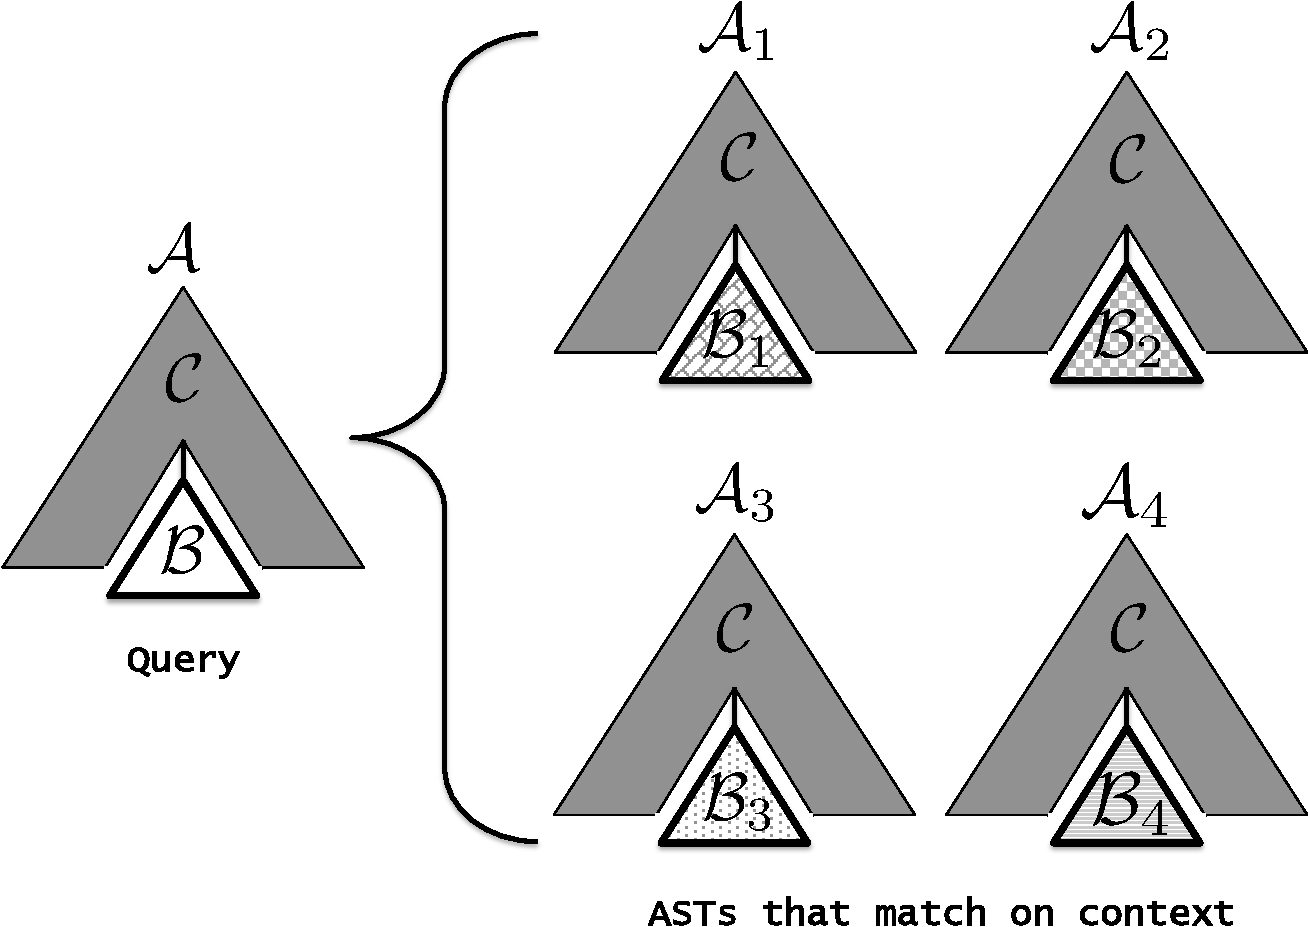
\includegraphics[width=.35\textwidth]{img/cartoon.pdf}
\caption{
Given a subtree $\mathcal{B}$ of an AST $\AST$, we query the Codewebs index
for other subtrees that also occur under the same context $(\AST\backslash\mathcal{B})$.
In this case, $\mathcal{B}_1, \dots, \mathcal{B}_4$ would each be considered
as candidates for the equivalence class of subtree $\mathcal{B}$ if the unit test outcomes for their
corresponding submissions matched that of the original AST $\AST$.
}
\label{fig:cartoon}
\end{figure}

\begin{enumerate}
\item {\bf Finding ``feet that fit the shoe''.}
\looseness -1 We perform a first pass to find candidate subtrees that are potentially equivalent to $\mathcal{B}$
by first detaching the subtree $\mathcal{B}$ from its surroundings, leaving the context $\mathcal{C} = \AST\backslash\mathcal{B}$.
We then query our index for the list of ASTs $\{\AST_1,\AST_2,\dots\}$ that contain $\mathcal{C}$ (See Figure~\ref{fig:cartoon}).

Under each retrieved AST $\AST_i$, the subtree $\mathcal{B}_i$ that is attached to the context $\mathcal{C}$ is
then considered to be a candidate for equivalence if $F[\AST_i] = F[\AST]$ (that is, if
the unit test outputs for the containing full AST $\AST_i$ agree with those of the original AST $\AST$). Intuitively, if another subtree shares the context $\mathcal{C}$ and 
produces the same output, it suggests that the two can be interchanged without affecting  functionality.

Before we add a new element to our set of equivalent subtrees 
we use the criterion proposed in Section~\ref{sec:testing} to verify that the new subtree is indeed
probabilistically equivalent to another subtree already in the set.
\item {\bf Finding ``shoes that fit the feet''.}
The first step will find all subtrees that have an exact context match with the originally annotated seed subtree. In order to expand our search for further equivalent subtrees, 
we then search for other contexts that can plausibly be attached to a subtree which is functionally equivalent to the seed. 

For each element $\mathcal{B}'$ in the set of equivalent subtrees found so far, we find all 
contexts that contain  $\mathcal{B}'$ and produce the same output as the program from 
which we found $\mathcal{B}'$. These contexts are hypothesized to also be attached to subtrees equivalent to the seed, 
and as such, represent new places to look for more potentially equivalent subtrees.
 
\item {\bf Repeat Until Convergence.}
We repeat steps (1) and (2) and expand both the set of equivalent subtrees as well as the
set of the contexts that we believe may be attached to one of the equivalent subtrees 
until the size of our set stops growing.
\end{enumerate}

\mypara{Reduction and reindexing}
Each equivalence class
$\Sigma=\{\mathcal{B}_1,\mathcal{B}_2,\dots\}$ 
learned from the data yields a set of canonicalization rules.  Thus whenever
we encounter a subtree $\mathcal{B}$ in an AST which happens to be a member of the equivalence class
$\Sigma$, we can replace $\mathcal{B}$ by a single member of that equivalence class (say, $\mathcal{B}_1$).
The identification of subtrees within an equivalence class
 leads to a reduction in the complexity of the collection of submitted ASTs since ASTs that were previously
distinct can now be transformed into the same tree.  Thus after finding an equivalence class, it is easier to expand a subsequent set.

\begin{figure}[t!]
\center
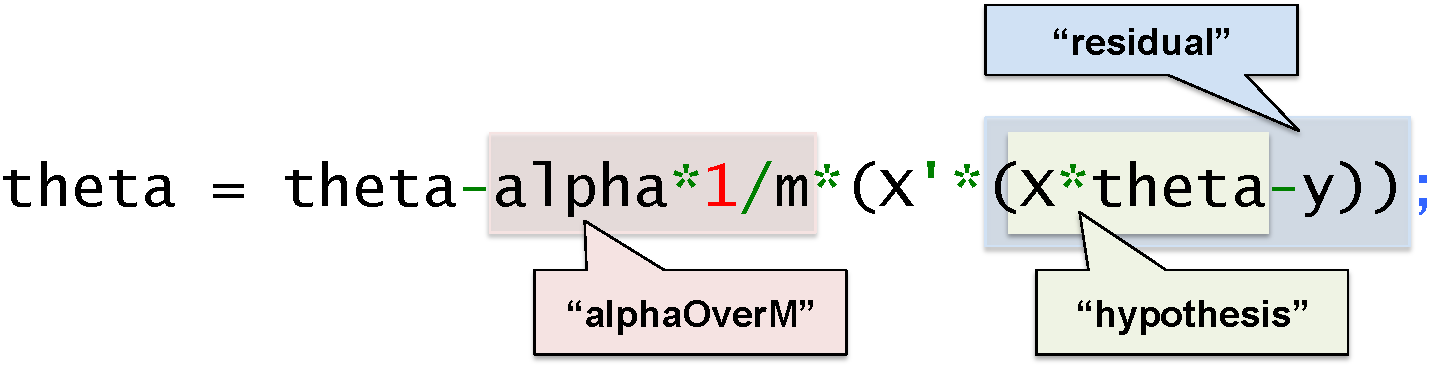
\includegraphics[width=.35\textwidth]{img/taggingexample.pdf}
\caption{
Example code snippets corresponding to AST subtrees tagged by an instructor for the linear regression problem.
}
\label{fig:tagging}
\end{figure}

\begin{figure}[t!]
\center
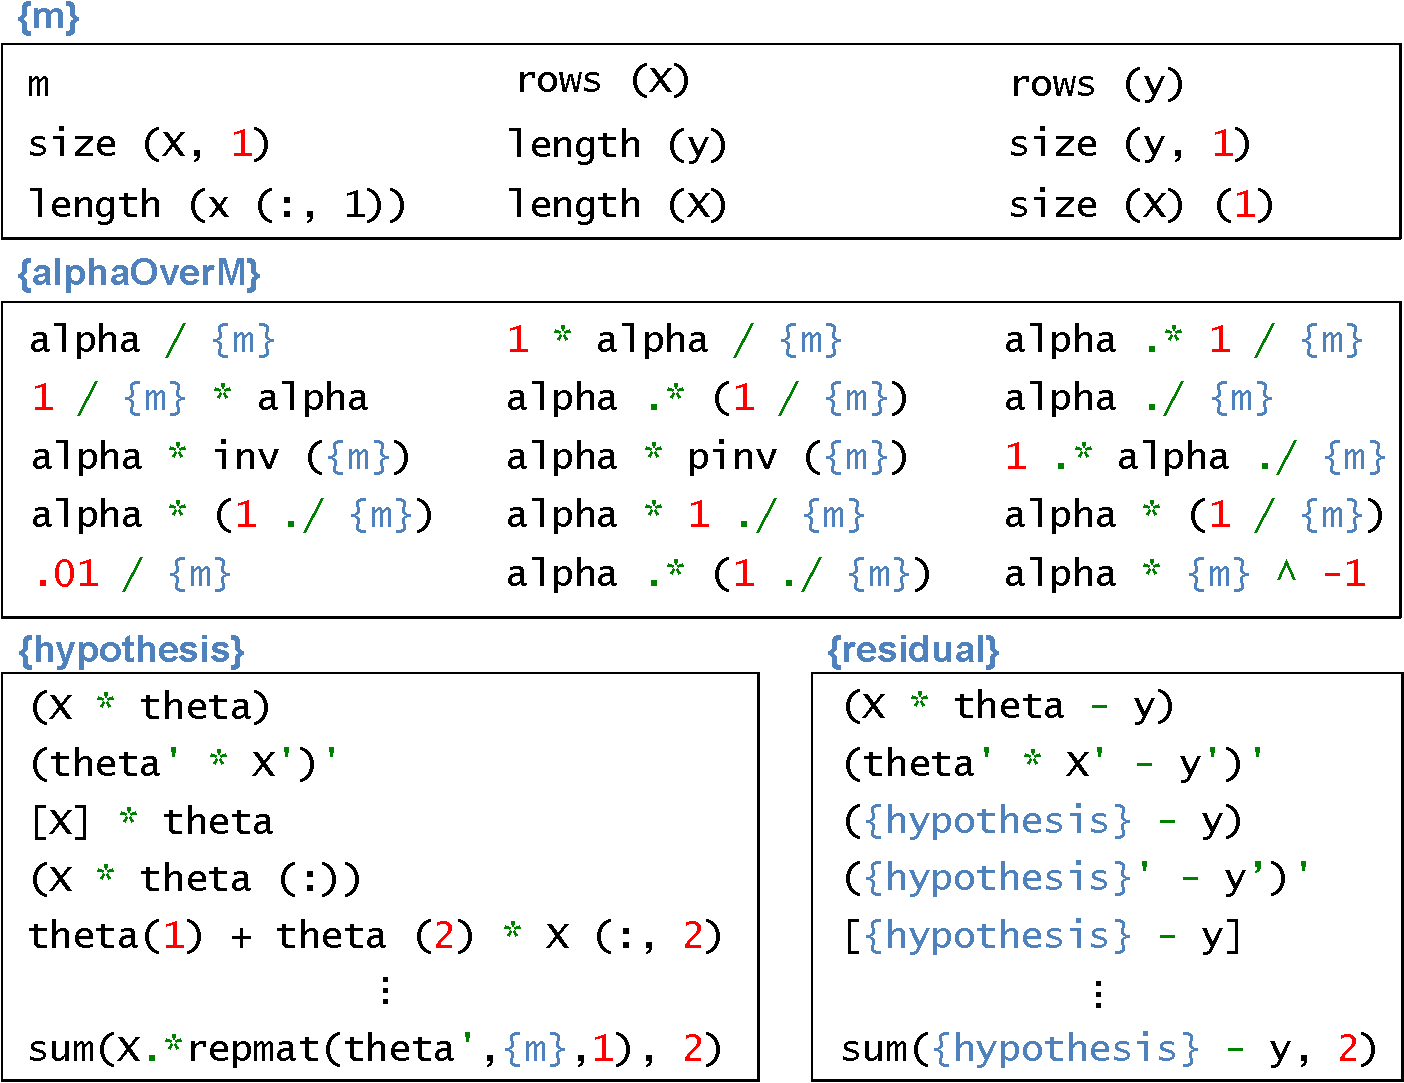
\includegraphics[width=.68\textwidth]{img/equivalencesAll.pdf}

\caption{
 Selections of code snippets algorithmically determined for the linear regression homework.  Note that not all subtrees from the equivalence classes are shown.
}
\label{fig:equivalences}
\end{figure}

\begin{example}
We highlight several examples of equivalence classes that were automatically discovered from the 
submissions to the linear regression problem (shown in Figure~\ref{fig:equivalences} with names in braces).  
Equivalence class $\{m\}$, for example, shows that $\texttt{length(y)}$ and $\texttt{size(y,1)}$ are equivalent, as discussed in Example~\ref{ex:lengthy}.
Note that equivalence classes can be defined in terms of other equivalence classes.

It would be difficult to imagine more than a handful of ways to write the expression $\texttt{alpha/m}$, 
but our algorithm was able to find 135 distinct AST subtrees in the equivalence class $\{\mbox{alphaOverM}\}$.
Note in particular that nearly all of the equivalences 
are not truly semantically equivalent in the strictest sense of Definition~\ref{def:exactequivalence}, but only
in the context of the homework problem.   For example, $\texttt{alpha/m}$ is not interchangeable
with $\texttt{.01/m}$ in general Octave programs, but since $\texttt{alpha}$ was set to be $.01$ for the linear
regression problem, the equivalence was valid in the sense of Definition~\ref{def:equivalence}.
 %Our equivalences do make assumptions which might not always be true even in the context of homework assignments. 
Similarly, we inferred an equivalence between the subtrees $\texttt{inv(m)}$ and $\texttt{1./m}$, which would 
not have been equal if a student had redefined $\texttt{m}$ to be a matrix instead of a scalar.
%The appearance of the subtree $\texttt{(X*theta - y) .* X(:, 1)}$ in Figure~\ref{fig:residual} may seem mysterious --- 
%but it can be explained by the fact that many students assumed the precondition that the first column of the input
%matrix $\texttt{X}$ (i.e., $\texttt{X(:,1)}$), was an all-ones vector (a correct assumption for this particular problem). Discovering these equivalences would be impossible with a small dataset, but with a MOOC-scale dataset, is indeed feasible.
\end{example}


\looseness -1 After the determination of each equivalence class, we rebuild the Codewebs index and optionally
identify further equivalences.  It is often the case that recognizing an equivalence class  $\mathcal{E}$ (and reindexing 
taking $\mathcal{E}$ into account) can help us to discover further equivalence classes.
For example, it might be the case that we do not 
initially have enough observations to conclude with sufficient statistical confidence that 
$\texttt{X*theta-y}$ can be rewritten equivalently as the expression $\texttt{-(y-(theta'*X')')}$.
However, by first identifying that $\texttt{X*theta}$ can be rewritten as $\texttt{(theta'*X')'}$, 
we are likely to find more matches in the database when querying for $\texttt{X*theta-y}$ and $\texttt{-(y-(theta'*X')')}$, respectively,
resulting in a larger sample size from which to draw conclusions.
Using the same insight that we leveraged to find equivalence classes, we can also create a class of \emph{attempts} 
to pair with every equivalence class, where attempts are defined to be
subtrees that fit into the same contexts as members of the equivalence class but change the output from correct to incorrect.
%\Jon{note that collapsing some equivalences can help further ones to be discovered.}

\section{Bug finding from search queries}
Since the input to our system includes unit test outputs, determining whether a code submission contains a bug is not a difficult problem.  However, determining where the bug lies is considerably more challenging.  We discuss a way to use the search engine to localize a bug within code solely by examining its AST.  In the next section we will justify its effectiveness by evaluating its ability to determine the presence of a bug in a query code submission \emph{without} having access to the unit test output of the query.

\mypara{Approach}
As our ultimate goal is to provide useful feedback to as many students as possible, we will focus on common, localizable bugs.  If we consider the distribution of unit test outputs of ASTs which contain a particular subtree, we would expect that such a distribution corresponding to a buggy subtree would be skewed towards incorrect outputs, while that corresponding to a non-buggy subtree would resemble the overall distribution of unit test outputs.  
As long as the subtrees are sufficiently small and the bugs sufficiently common, it is possible to have a reliably large sample of these unit test
output distributions to use for the purposes of classification.

Notice, however, that as the subtrees become larger, the corresponding sample sizes necessarily decrease.  In fact, for any submission not in our training set, the improper subtree consisting of the full AST must has a unit test output distribution with sample size zero.  Thus to increase the sample sizes of our distributions, we use distributions corresponding to local contexts instead of subtrees for classification.

\mypara{Algorithm}
Our algorithm consists of an indexing phase and a query phase.  In the indexing phase, we iterate over the local contexts of all proper subtrees of all ASTs in our collection.  For each unique local context we construct a histogram of the unit tests outputs of the ASTs to which the context belongs.   Notice that these histograms
can be built via queries to our index described in Section~\ref{sec:indexing}.
We then classify each local context as being either buggy or not buggy based on the skew and sample size of its unit test output histogram.

In the query phase, we iterate over the local contexts of all proper subtrees of a query AST.  For each local context $\parentsubtree\backslash\subtree$ we mark node $\parent$ if the local context is recognized as 
buggy by our index.  We then unmark any node with a marked descendant, and report all remaining marked nodes as the roots of the buggy subtrees.

%\subsection{Bug identification by reduction}
%\mypara{Building a bug database}
%\subsection{Statistical bug isolation}

\begin{figure}[t!]
\center
\subfigure[]{
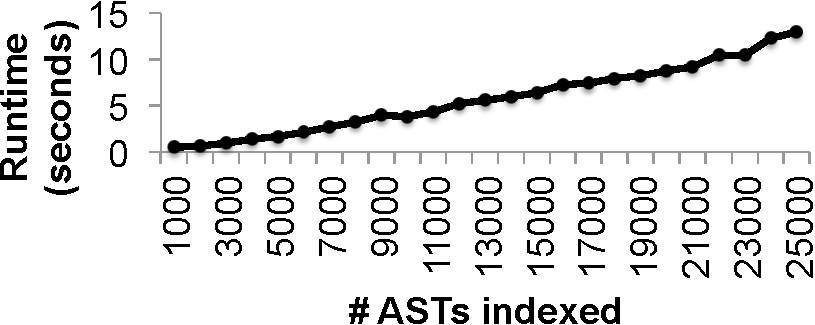
\includegraphics[width=.475\textwidth]{img/numastsvsruntime.pdf}
\label{fig:numastsvsruntime}
}
\subfigure[]{
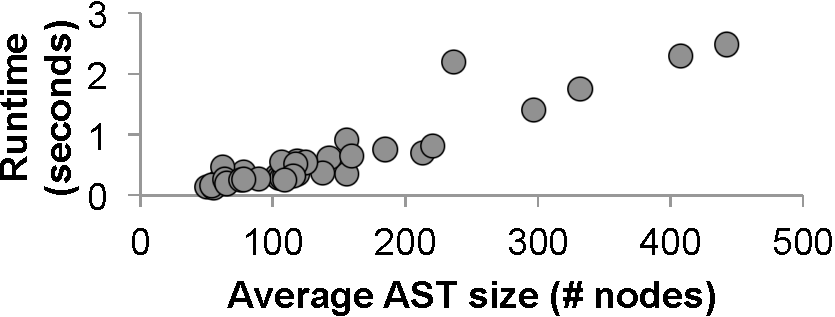
\includegraphics[width=.475\textwidth]{img/astsizevsruntime.pdf}
\label{fig:astsizevsruntime}
}

\caption{\subref{fig:numastsvsruntime} Runtime in seconds for indexing a collection of ASTs (as a function of the number of ASTs)
from the ``gradient descent (for linear regression)'' problem;
\subref{fig:astsizevsruntime} Runtime in seconds for indexing 1000 ASTs from each of the homework problems for Coursera's ML course plotted
against average AST size (\# nodes) for each problem}
%\label{fig:numastsvsruntime}
\end{figure}
\begin{figure*}[t!]
\center
\subfigure[]{
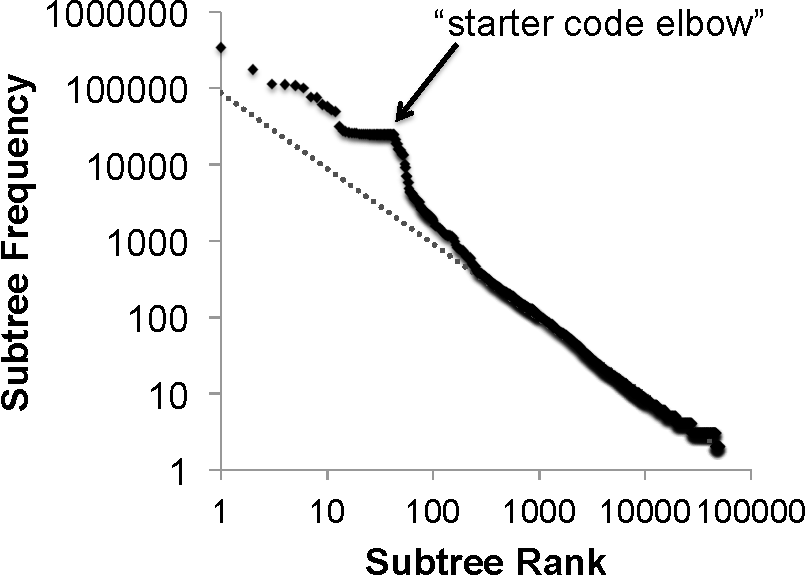
\includegraphics[width=.30\textwidth]{img/zipfnoequivalence.pdf}
\label{fig:zipfnoequiv}
}
\subfigure[]{
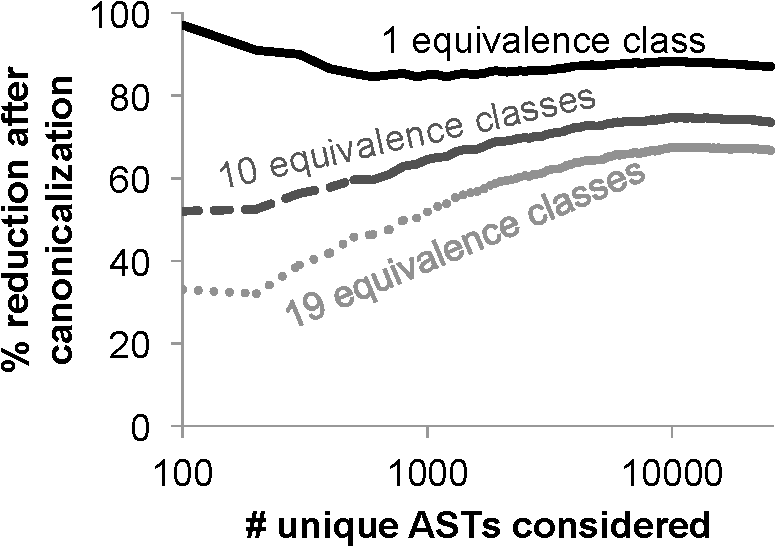
\includegraphics[width=.30\textwidth]{img/reduction.pdf}
\label{fig:reduction}
}
\subfigure[]{
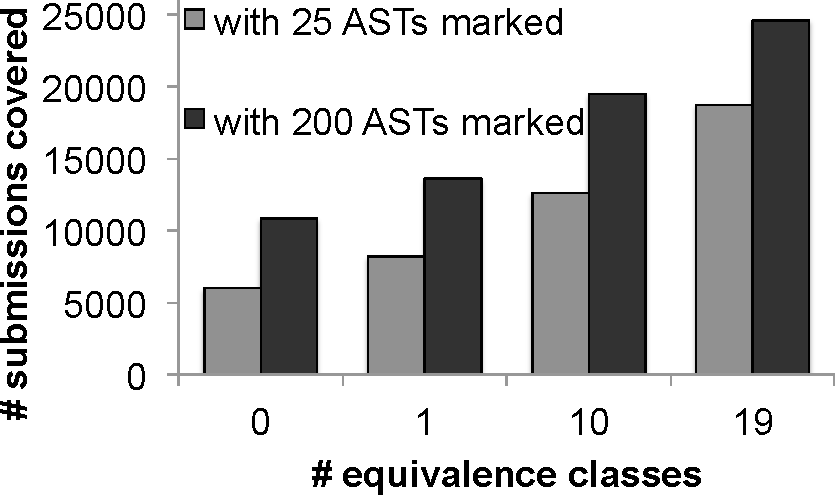
\includegraphics[width=.30\textwidth]{img/reduction2.pdf}
\label{fig:reduction2}
}

\caption{
\subref{fig:zipfnoequiv}
Zipf's Law: subtree frequency plotted against subtree rank (in the frequency table). % with and without canonicalization.  
%Note that our data closely follows Zipf's law (dotted line) except at an ``elbow'' at the top of the ranked list.
%We do not include time required for parsing or loading ASTs from disk in the above plot.
%Note that this is eclipsed by time for parsing (roughly 2 hours for all 40790 submissions).
\subref{fig:reduction} Fraction of remaining unique ASTs after canonicalizing the $k$ most frequent ASTs with 1, 10 or 19 learned equivalence classes;
\subref{fig:reduction2} Number of submissions covered if an instructor were to mark the 25 or 200 most frequent ASTs after canonicalization
}

\label{fig:zipfreduction}
\end{figure*}

\section{Empirical findings}\label{sec:evaluation}
In this section we present  empirical studies
of the performance of our Codewebs system and use it to study data from Stanford's ML class.
Our current implementation uses a parser (adapted from the Octave project~\cite{eaton97}) to convert
submitted source code to ASTs.   The Codewebs indexer can be run on a personal
computer with the full index fitting in under 6Gb of main memory for almost all problems.
Our running time tests were run on a %  \Jon{andy's machine}
Lenovo Thinkpad 
%W520 Intel Core i7-2760QM CPU 
(2.40 GHz) with 8 GB RAM.


\mypara{Running time}
We first consider the amount of time required for indexing 
by plotting the running time 
 as a function of the number of ASTs (for the linear regression problem).
We index only the uncanonicalized ASTs for this plot, though in general we iterate through multiple stages of indexing
as new equivalence classes are discovered.
In Figure~\ref{fig:numastsvsruntime}, we see that indexing the full set of ASTs requires roughly 16 seconds, excluding the time required for loading the ASTs 
from disk (which can dominate indexing time, depending on the platform).  

We next show how the indexing time scales as a function of the number of nodes in an AST.
Figure~\ref{fig:astsizevsruntime} plots the running time required to index 1000 ASTs 
on forty different programming problems against the average number of nodes per AST for each problem.
%We observe running time to be 
%(slightly) superlinear in the size of the AST due to the quadratic
%number of subforests (which is more apparent for problems with long statement lists).

%\Jon{no local contexts built here.}
%\Jon{time for discovering equivalence classes, }
%\begin{itemize}\denselist
%\item How much time do we need to reduce a set of ASTs?
%\item Running time as a function of the number of ASTs provided
%\item Running time as a function of AST size
%\end{itemize}

We finally note that in all cases, the combined time for all parsing, indexing, and equivalence discovery operations
is dominated by the amount of time that students are given to complete an assignment (consisting of 5-7 programming problems on average).

\mypara{Code phrase statistics}
Given the scale of our data, it is natural to ask:  \emph{have we seen all of the code phrases that we are likely to see?}
For insight, we turn to Zipf's law~\cite{zipf1949human}, which characterizes a phenomenon that
 the frequency of a word in a large scale natural language corpus
is inversely proportional to its rank in the frequency table. 
Thus a few words might be used millions of times,
but many words are just used once. 
Zipf's law has had implications for search engine design, particular for efficient index compression and caching~\cite{breslau99}.
Among other things, we know that when words are sampled from a Zipfian distribution, the size of the vocabulary grows
indefinitely without converging to a fixed maximum size~\cite{lu10}.

Asking the similar question of whether code phrases also obey such a law may yield
insight into how the Codewebs index is expected to grow as a function of the size of the dataset of submissions.
Due to the constrained nature of the data, we might expect significantly 
less variety in code phrases than in natural language.  However, our data tells another story: Figure~\ref{fig:zipfnoequiv},
plots the frequency of a subtree against its corresponding rank in the frequency table.  This frequency table was constructed 
from all subtrees taken from 10,000 distinct ASTs submitted to the linear regression problem.
The relationship between the log rank and log frequency is evidently nearly linear
 with an ``elbow'' at around the $45^{th}$ most frequent subtree, up to which all earlier subtrees occur more than 10,000 times.  
 We hypothesize that this elbow is due to the subtrees included in the provided starter code that was shared by almost all implementations.

A linear regression shows that $\log (\texttt{rank}) \approx a- b\cdot\log (\texttt{freq})$, where $a=10.677$
and $b=1.01$ (which is remarkably close to the slope of 1 postulated by Zipf's law). 
Thus given a subtree from a new submission, there is a significant probability that it has not yet 
been observed in the data.  On the other hand, the result also suggests that prior work on dealing with large scale traditional indexing may apply to
scaling up code phrase indexing as well.
%\Jon{and with equivalences?}

\mypara{Equivalence classes and reduction}
We now evaluate the amount of reduction obtained via canonicalization.  We 
manually tagged 19 code phrases that were likely to vary in the linear regression problem (including those shown in Figure~\ref{fig:equivalences})
and used the Codewebs engine to thus find 19 equivalence classes.
We first examine the reduction factor in the number of distinct ASTs
if applying canonicalization to the $k$ most frequently submitted ASTs.
Figure~\ref{fig:reduction} shows the result when canonicalizing with just one equivalence
class, with 10 equivalence classes, and all 19.  We see that using more equivalence classes
helps for reduction, and in general, we observe better reduction factors among the more popular
ASTs compared to that of the the overall dataset.

We can also examine the number of submissions that an instructor could ``cover'' by giving feedback only to
the $k$ most frequent ASTs (rather than the entire set of ASTs).\footnote{
As we discuss later in this section (the \emph{Feedback case study}), we would more typically  mark code phrases rather than full ASTs,
which would in general lead to greater coverage of students.}
Figure~\ref{fig:reduction2} plots the achieved coverage if an instructor were to mark 25 ASTs or 200 ASTs
after using canonicalization (again with varying numbers of equivalence classes).
Unsurprisingly, the instructor increases coverage simply by marking more ASTs.  However,
the plots also suggest that canonicalizing has even more of an impact on coverage --- we cover nearly 25,000
of the roughly 40,790 submissions to the linear regression problem by marking 200 canonicalized ASTs.
Note that we also cover 73\% more submissions by marking just 25 canonicalized ASTS than 
if we were to mark 200 uncanonicalized ASTs.

\mypara{Bug identification}
Evaluating bug localization is challenging since there is currently no available ``ground truth'' data
on the locations of bugs in submitted code.  We thus only evaluate our ability to detect
the presence of a bug in a submission (instead of requiring localization), for which we do have ground truth through unit tests.
Using a $\mbox{Beta}(0.1, 0.1)$ prior on the probability of an AST having no bugs, 
we train our detector in leave-one-out fashion, evaluating accuracy of predicting the presence of a bug 
%(using F-score) 
on the left out example.  
As a baseline, we compare against a $k$-nearest neighbor classifier based on tree edit distance between
ASTs with $k=5$ (see our previous work,~\cite{huang13}).  



\begin{figure}[t!]
\center
%\subfigure[]{
%\includegraphics[width=.30\textwidth]{img/bugsComparison.pdf}
%\label{fig:bugsAll}
%}\;
\subfigure[]{
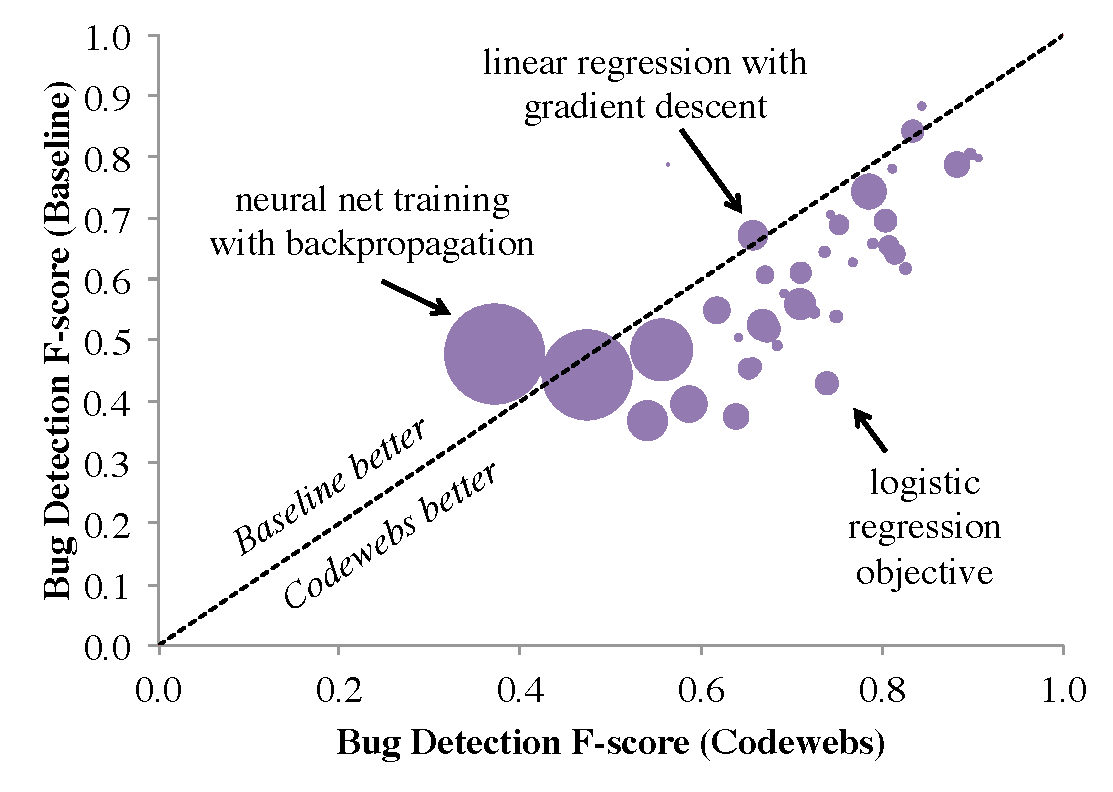
\includegraphics[width=.31\textwidth]{img/bugsFscoreDiffs.pdf}
\label{fig:bugsAll}

}
\qquad\qquad
\subfigure[]{
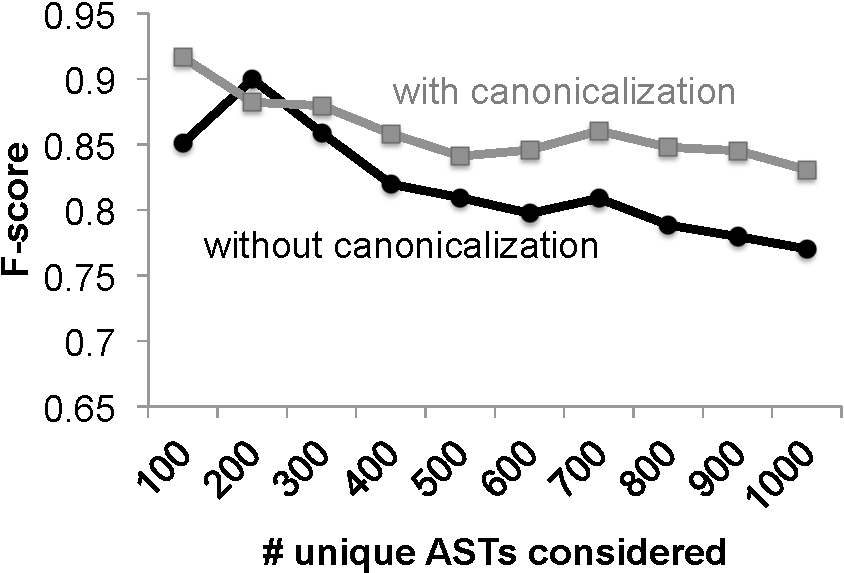
\includegraphics[width=.3\textwidth]{img/bugIsolation.pdf}
\label{fig:bugIsolation}
}

\caption{
\subref{fig:bugsAll}  F-score comparison of Codewebs based bug detection algorithm against baseline (5-nearest neighbors) 
for the 5000 most frequent ASTs for each assigned homework problem.  Each circle corresponds to a single homework problem, 
with circle widths  set to be proportional to the average \# of nodes per AST for that problem; 
\subref{fig:bugIsolation} Codewebs based bug detection F-scores on the $k$ most frequent ASTs, with and without canonicalization
on the ``linear regression with gradient descent'' homework problem.
}
\label{fig:exp2}
\end{figure}


Considering buggy programs as positive examples, we evaluate the precision and recall
of both classifiers on the 5000 most frequent ASTs for each homework problem in the class
and compute the \emph{F-score} (i.e., the harmonic mean of precision and recall, with higher values
corresponding to higher accuracy) in each case.
Figure~\ref{fig:bugsAll} compares this F-score performance of our query based bug detection
algorithm against that of $k$NN.   As a rough measure of problem complexity, we also visualize
 the average number of nodes per AST in each problem (after subtracting
the number of AST nodes that come from the provided starter code) by varying circle sizes.
As can be seen in the plot, bug detection is generally more difficult for both approaches on the more
complex assignments, with the neural network training problems being the most difficult.
%Points below the diagonal in this plot correspond to homework problems
%on which our Codewebs based bug detector outperforms the baseline algorithm.
However in many problems, we obtain reasonable accuracy using both approaches with
the Codewebs based algorithm outperforming the baseline in most cases.

%Our algorithm is successful with most points lying in the upper right corner of the scatter plot.
%The two problems on which our algorithm had the most difficulty were related to the neural network backpropagation assignment,
%in which the submitted implementations were significantly lengthier than those of other problems (with over 40 lines of code per implementation).

%To show that our algorithm performs the best for the most frequently submitted ASTs,
Figure~\ref{fig:bugIsolation} plots the performance  of our detection algorithm
on the 100 most frequent ASTs, 200 most frequent, and so on for the linear regression problem.
As in our reduction experiments, performance is better 
for the more frequently submitted ASTs, and the drop in accuracy as we get to less frequent ASTs is graceful.
Using canonicalization again helps to boost performance in general.
On 1000 ASTs, our bug detection precision (with canonicalization) is .78 and recall is .88.
Finally, we remark that the bug localization algorithm is fast and capable of  handling over 150 requests per second (for the
linear regression problem with an average AST size 116).

\mypara{Feedback case study}
Without the help of our system, the easiest way to scalably provide feedback to students in a MOOC is to 
send canned feedback for the most frequent (incorrect) unit test outcomes, which often reflect common misunderstandings.
One weakness of this unit-test based approach, however, is that it can fail when a single conceptual misunderstanding
can lead to multiple unit test outcomes, or when it occurs in the presence of other bugs.
We  illustrate  how the Codewebs system can be used to give feedback to students even
when the unit-test based approach fails.

In the linear regression problem, many students
erroneously included an ``extraneous sum'' in the gradient expression
(e.g., with $\texttt{sum((X*theta-y)'*X)}$ instead of   $\texttt{X'*(X*theta-y)}$ ). 
Upon identifying a single instance of the bug, an instructor can then use
the Codewebs system 
to extract many equivalent ways of writing the erroneous expression (e.g., $\texttt{sum(((theta'*X')'-y)'*X)}$, $\texttt{sum(transpose(X*theta-y)*X)}$, etc.).   
These expressions are then matched to incoming student submissions, for which we can
provide a human generated message explaining the cause of the misunderstanding.

After extracting equivalences and matching to the existing submissions, our algorithm
found 1208 submissions which matched the ``extraneous sum'' bug, outperforming a unit test based
feedback strategy which would have covered 1091 submissions.  We can also use both strategies together, giving feedback to submissions found by either
method to contain the bug, 
which would lead to a 47\% increase in number of submissions covered over just using unit tests.

\section{Related work}\label{sec:relatedwork}
Our paper builds upon a body of work on reasoning with code collections --- a problem that arises
both for programmers and for those learning to program.  
Code search engines, many of which scale to massive databases 
have been proposed, for example, for the purposes of code reuse or navigating a complicated API~\cite{sindhgatta06,hoffmann07}.
A number of choices exist in this domain of reasoning with a code collection.
How much structure to take into account is one such choice, 
with some systems reasoning at the level of keywords or tokens~\cite{hummel08, hartmann10} to other systems reasoning
with the full syntactic 
structure of the AST~\cite{paul94, thummalapenta07,kim10}.
Canonicalization has been a popular approach for reducing the variance of a large collection of code  in many such works~\cite{baxter98,xu03}.
In contrast to our paper, this work on code search engines generally has focused on helping programmers to understanding what tools in an existing 
codebase can help a programmer to accomplish 
a certain task, which is reflected by features that are commonly supported, such as the ability to query for usage examples for a function, 
or to find methods that require a certain type as a parameter.  
Closer to our setting is the work of Rivers et al.~\cite{rivers12,rivers13}, who also used ASTs with canonicalization to map out the solution space to 
introductory programming problems and discover common errors.

However, reasoning about function is critical in many settings, and thus
another choice that has received recent attention is whether to incorporate 
unit test information~\cite{hummel08,lazzarini09}.  
Our work efficiently combines what we believe to be the best of the above ideas: reasoning with ASTs and unit tests, as well as combining the
two sources of data to automatically discover semantically equivalent code phrases.  To our knowledge, this is
the first method for automatically finding canonicalization rules for programs.

%Reasoning with a collection of code for educational purposes is a more recent topic which we
%predict will become more prevalent in the literature as MOOC datasets become more widely available 
%to researchers.

The idea that student code can be ``clustered'' into a small category of approaches has also been explored by a number of researchers.
Piech et al.~\cite{piech12}, for example, cluster trajectories of ASTs over multiple submits by a single student.  
Glassman et al.~\cite{glassman13} visualize the space of student solutions to Matlab programming problems in order to identify popular approaches for
solving a problem.
A number of recent papers have clustered students based on abstract syntax trees using distances in feature 
space~\cite{gross12,gross13}, string edit distance~\cite{rivers12,rivers13}
and tree edit distance~\cite{huang13}, proposing to give feedback to exemplar submissions.	
These methods rely almost completely on syntactic analysis and do not 
explicitly relate form to function as in our work. Furthermore, for assignments with multiple ``parts'', each of which can be approached in multiple ways, 
the number of clusters intuitively can grow exponentially in the number of parts, leading to a loss of interpretability and effectiveness of the method.
Our work is the first to explicitly address the idea that smaller parts of code can be shared among submissions.

\section{Discussion}\label{sec:discussion}
MOOC platforms now collect massive datasets of student submissions across hundreds of courses, 
introducing new research problems of how to organize and search the data 
effectively, but also new opportunities to use the data in ways that were not previously possible.
We have developed a system called Codewebs which efficiently indexes all of the code submissions to a 
MOOC programming assignment and can be useful in a number of applications.  
Through a novel use of unit test information, our system is also able to determine 
when code snippets are semantically equivalent in a data driven way.

As the MOOC ecosystem continues to quickly expand, it is crucial for 
accompanying learning technologies to be applicable to a large variety of courses with minimal effort on the part of the instructor.
Codewebs makes no assumptions about the underlying assignments and is designed to be easily applicable to a 
wide variety of programming languages.
Instead of running dynamic analysis on fully instrumented programs, the system relies only on unit test information
which is lightweight and thus contributes to portability.
To apply Codewebs to a programming problem, the most important requirement is a large dataset of student submissions (which is a given in MOOCs).
Beyond data, we only have a handful of requirements:
(1) a mechanism for parsing source code into an abstract syntax tree (which is available for most programming languages)
(2) a specification of which nodes of an AST correspond to statements, identifiers, and constants, 
(3) a listing of reserved functions and identifiers that are not to be anonymized, 
(4) sufficiently informative unit tests for problems, and 
(5) instructor specified
points of variation for determining canonicalization rules.  
Thus we believe that applying the Codewebs system to submissions in other coding intensive courses should be straightforward.

There are a number of directions ripe for future work.
At the moment, our system only handles code that parses correctly.  However for beginning programmers,
even writing syntactically valid code can be a challenge.  Thus the question of how to leverage a large
dataset for giving feedback to unparseable submissions remains an important open problem.  
Our current approach is also limited to indexing submissions of a single function where all implementations receive
the same input and thus can be unit tested in a unified way.
Thus another open problem is how to deal with long form programs in which
students are free to choose how to decompose an implementation into smaller modules.

We believe  many of the insights that went into creating the Codewebs system
may also apply to general search engines for source code outside of the educational setting. 
But more interestingly, these ideas may also apply to indexing formal logic proofs~\cite{fast13} and equations~\cite{kohlhase06}, or even 
natural language mathematical proofs, which can be useful either for researchers or educators.
%or in math and statistics courses offered online.
Looking even further, it is tantalizing to speculate about the role that effective search engines for student content
 might play in the MOOC ecosystem beyond STEM (science, technology, engineering and mathematics) courses. 
Public exhibitions of student work are, for example, a common way to culminate university level art and design courses --- but 
pulling these exhibitions off at the scale of MOOCs requires an effective way to search through tens of thousands of submissions.
And while the specific features of designing a search engine for one of these courses will surely be different from the Codewebs
setting,  many of the same questions will still apply.  
What are the natural queries for an assignment?
How can we exploit the organizational structure of a search engine index to facilitate student feedback?
How do we scale to tens of thousands of students?

\subsection*{Acknowledgments}

We thank Andrew Ng, Daphne Koller, John Mitchell, and Mehran Sahami for 
useful conversations.
%J. Huang is supported by an NSF Computing Innovations Fellowship 
%and C. Piech is supported by an NSF Graduate Fellowship.
This research was funded by
NSF grants CCF 1011228 and  DMS 1228304, AFOSR grant FA9550-12-1-0372,  a Google Research Award, and the Max Planck Center for Visual Computing and Communications.
J. Huang is supported by the CRA CI Fellows grant 104672, and C. Piech by the NSF